% Options for packages loaded elsewhere
\PassOptionsToPackage{unicode}{hyperref}
\PassOptionsToPackage{hyphens}{url}
%
\documentclass[
  man,floatsintext]{apa6}
\usepackage{amsmath,amssymb}
\usepackage{iftex}
\ifPDFTeX
  \usepackage[T1]{fontenc}
  \usepackage[utf8]{inputenc}
  \usepackage{textcomp} % provide euro and other symbols
\else % if luatex or xetex
  \usepackage{unicode-math} % this also loads fontspec
  \defaultfontfeatures{Scale=MatchLowercase}
  \defaultfontfeatures[\rmfamily]{Ligatures=TeX,Scale=1}
\fi
\usepackage{lmodern}
\ifPDFTeX\else
  % xetex/luatex font selection
\fi
% Use upquote if available, for straight quotes in verbatim environments
\IfFileExists{upquote.sty}{\usepackage{upquote}}{}
\IfFileExists{microtype.sty}{% use microtype if available
  \usepackage[]{microtype}
  \UseMicrotypeSet[protrusion]{basicmath} % disable protrusion for tt fonts
}{}
\makeatletter
\@ifundefined{KOMAClassName}{% if non-KOMA class
  \IfFileExists{parskip.sty}{%
    \usepackage{parskip}
  }{% else
    \setlength{\parindent}{0pt}
    \setlength{\parskip}{6pt plus 2pt minus 1pt}}
}{% if KOMA class
  \KOMAoptions{parskip=half}}
\makeatother
\usepackage{xcolor}
\usepackage{graphicx}
\makeatletter
\def\maxwidth{\ifdim\Gin@nat@width>\linewidth\linewidth\else\Gin@nat@width\fi}
\def\maxheight{\ifdim\Gin@nat@height>\textheight\textheight\else\Gin@nat@height\fi}
\makeatother
% Scale images if necessary, so that they will not overflow the page
% margins by default, and it is still possible to overwrite the defaults
% using explicit options in \includegraphics[width, height, ...]{}
\setkeys{Gin}{width=\maxwidth,height=\maxheight,keepaspectratio}
% Set default figure placement to htbp
\makeatletter
\def\fps@figure{htbp}
\makeatother
\setlength{\emergencystretch}{3em} % prevent overfull lines
\providecommand{\tightlist}{%
  \setlength{\itemsep}{0pt}\setlength{\parskip}{0pt}}
\setcounter{secnumdepth}{-\maxdimen} % remove section numbering
% Make \paragraph and \subparagraph free-standing
\ifx\paragraph\undefined\else
  \let\oldparagraph\paragraph
  \renewcommand{\paragraph}[1]{\oldparagraph{#1}\mbox{}}
\fi
\ifx\subparagraph\undefined\else
  \let\oldsubparagraph\subparagraph
  \renewcommand{\subparagraph}[1]{\oldsubparagraph{#1}\mbox{}}
\fi
% definitions for citeproc citations
\NewDocumentCommand\citeproctext{}{}
\NewDocumentCommand\citeproc{mm}{%
  \begingroup\def\citeproctext{#2}\cite{#1}\endgroup}
\makeatletter
 % allow citations to break across lines
 \let\@cite@ofmt\@firstofone
 % avoid brackets around text for \cite:
 \def\@biblabel#1{}
 \def\@cite#1#2{{#1\if@tempswa , #2\fi}}
\makeatother
\newlength{\cslhangindent}
\setlength{\cslhangindent}{1.5em}
\newlength{\csllabelwidth}
\setlength{\csllabelwidth}{3em}
\newenvironment{CSLReferences}[2] % #1 hanging-indent, #2 entry-spacing
 {\begin{list}{}{%
  \setlength{\itemindent}{0pt}
  \setlength{\leftmargin}{0pt}
  \setlength{\parsep}{0pt}
  % turn on hanging indent if param 1 is 1
  \ifodd #1
   \setlength{\leftmargin}{\cslhangindent}
   \setlength{\itemindent}{-1\cslhangindent}
  \fi
  % set entry spacing
  \setlength{\itemsep}{#2\baselineskip}}}
 {\end{list}}
\usepackage{calc}
\newcommand{\CSLBlock}[1]{\hfill\break\parbox[t]{\linewidth}{\strut\ignorespaces#1\strut}}
\newcommand{\CSLLeftMargin}[1]{\parbox[t]{\csllabelwidth}{\strut#1\strut}}
\newcommand{\CSLRightInline}[1]{\parbox[t]{\linewidth - \csllabelwidth}{\strut#1\strut}}
\newcommand{\CSLIndent}[1]{\hspace{\cslhangindent}#1}
\ifLuaTeX
\usepackage[bidi=basic]{babel}
\else
\usepackage[bidi=default]{babel}
\fi
\babelprovide[main,import]{english}
% get rid of language-specific shorthands (see #6817):
\let\LanguageShortHands\languageshorthands
\def\languageshorthands#1{}
% Manuscript styling
\usepackage{upgreek}
\captionsetup{font=singlespacing,justification=justified}

% Table formatting
\usepackage{longtable}
\usepackage{lscape}
% \usepackage[counterclockwise]{rotating}   % Landscape page setup for large tables
\usepackage{multirow}		% Table styling
\usepackage{tabularx}		% Control Column width
\usepackage[flushleft]{threeparttable}	% Allows for three part tables with a specified notes section
\usepackage{threeparttablex}            % Lets threeparttable work with longtable

% Create new environments so endfloat can handle them
% \newenvironment{ltable}
%   {\begin{landscape}\centering\begin{threeparttable}}
%   {\end{threeparttable}\end{landscape}}
\newenvironment{lltable}{\begin{landscape}\centering\begin{ThreePartTable}}{\end{ThreePartTable}\end{landscape}}

% Enables adjusting longtable caption width to table width
% Solution found at http://golatex.de/longtable-mit-caption-so-breit-wie-die-tabelle-t15767.html
\makeatletter
\newcommand\LastLTentrywidth{1em}
\newlength\longtablewidth
\setlength{\longtablewidth}{1in}
\newcommand{\getlongtablewidth}{\begingroup \ifcsname LT@\roman{LT@tables}\endcsname \global\longtablewidth=0pt \renewcommand{\LT@entry}[2]{\global\advance\longtablewidth by ##2\relax\gdef\LastLTentrywidth{##2}}\@nameuse{LT@\roman{LT@tables}} \fi \endgroup}

% \setlength{\parindent}{0.5in}
% \setlength{\parskip}{0pt plus 0pt minus 0pt}

% Overwrite redefinition of paragraph and subparagraph by the default LaTeX template
% See https://github.com/crsh/papaja/issues/292
\makeatletter
\renewcommand{\paragraph}{\@startsection{paragraph}{4}{\parindent}%
  {0\baselineskip \@plus 0.2ex \@minus 0.2ex}%
  {-1em}%
  {\normalfont\normalsize\bfseries\itshape\typesectitle}}

\renewcommand{\subparagraph}[1]{\@startsection{subparagraph}{5}{1em}%
  {0\baselineskip \@plus 0.2ex \@minus 0.2ex}%
  {-\z@\relax}%
  {\normalfont\normalsize\itshape\hspace{\parindent}{#1}\textit{\addperi}}{\relax}}
\makeatother

\makeatletter
\usepackage{etoolbox}
\patchcmd{\maketitle}
  {\section{\normalfont\normalsize\abstractname}}
  {\section*{\normalfont\normalsize\abstractname}}
  {}{\typeout{Failed to patch abstract.}}
\patchcmd{\maketitle}
  {\section{\protect\normalfont{\@title}}}
  {\section*{\protect\normalfont{\@title}}}
  {}{\typeout{Failed to patch title.}}
\makeatother

\usepackage{xpatch}
\makeatletter
\xapptocmd\appendix
  {\xapptocmd\section
    {\addcontentsline{toc}{section}{\appendixname\ifoneappendix\else~\theappendix\fi: #1}}
    {}{\InnerPatchFailed}%
  }
{}{\PatchFailed}
\makeatother
\keywords{proportional reasoning, visual formats, cognitive science\newline\indent Word count: X}
\usepackage{lineno}

\linenumbers
\usepackage{csquotes}
\ifLuaTeX
  \usepackage{selnolig}  % disable illegal ligatures
\fi
\usepackage{bookmark}
\IfFileExists{xurl.sty}{\usepackage{xurl}}{} % add URL line breaks if available
\urlstyle{same}
\hypersetup{
  pdftitle={Proportional Reasoning Across Formats},
  pdfauthor={Albert Sebastian1},
  pdflang={en-EN},
  pdfkeywords={proportional reasoning, visual formats, cognitive science},
  hidelinks,
  pdfcreator={LaTeX via pandoc}}

\title{Proportional Reasoning Across Formats}
\author{Albert Sebastian\textsuperscript{1}}
\date{}


\shorttitle{Proportional Reasoning}

\authornote{

The authors made the following contributions. Albert Sebastian: Conceptualization, Data Analysis, Writing - Original Draft Preparation.

Correspondence concerning this article should be addressed to Albert Sebastian, 123 Research Lane, Rutgers University. E-mail: \href{mailto:albert.sebastian@email.com}{\nolinkurl{albert.sebastian@email.com}}

}

\affiliation{\vspace{0.5cm}\textsuperscript{1} Rutgers University}

\abstract{%
Comparing proportions is a fundamental cognitive skill demonstrated across human development. This study examines how well adults compare proportions when presented in different visual formats. Here we show that performance varies significantly across formats, with integrated formats leading to higher accuracy. These results highlight the role of visual integration in proportional reasoning, advancing our understanding of how humans process comparative proportions. This study further demonstrates a positive correlation between reaction time and accuracy, providing insights into decision-making processes in perceptual tasks.
}



\begin{document}
\maketitle

\section{Introduction}\label{introduction}

Comparing proportions is a fundamental cognitive skill seen in infants and adults alike. However, the ability to do so can be influenced by how proportions are presented. Visual integration and congruency play critical roles in making accurate judgments. This study seeks to explore the impact of presentation formats and numerator congruency on proportional reasoning, with the following objectives:\\
1. Does average performance vary across format type?\\
2. Does average performance vary across numerator congruency status?\\
3. Does numerator congruency vary across format type? (i.e., is there an interaction)\\
This investigation expands on prior work by examining the relationship between reaction time and accuracy, providing new insights into decision-making processes in proportional reasoning tasks.

\section{Methods}\label{methods}

A total of 99 adults participated in the study.

First, participants were introduced to a story about a magic ball and that the outcome (i.e., blue or orange) depended on the proportions. They were then asked to compare the proportions of different images. In other words, participants were shown two images of the same kind at the same time and asked to decide which had a higher proportion of the shape (or dots) colored in blue.

\begin{figure}[H]
  \centering
  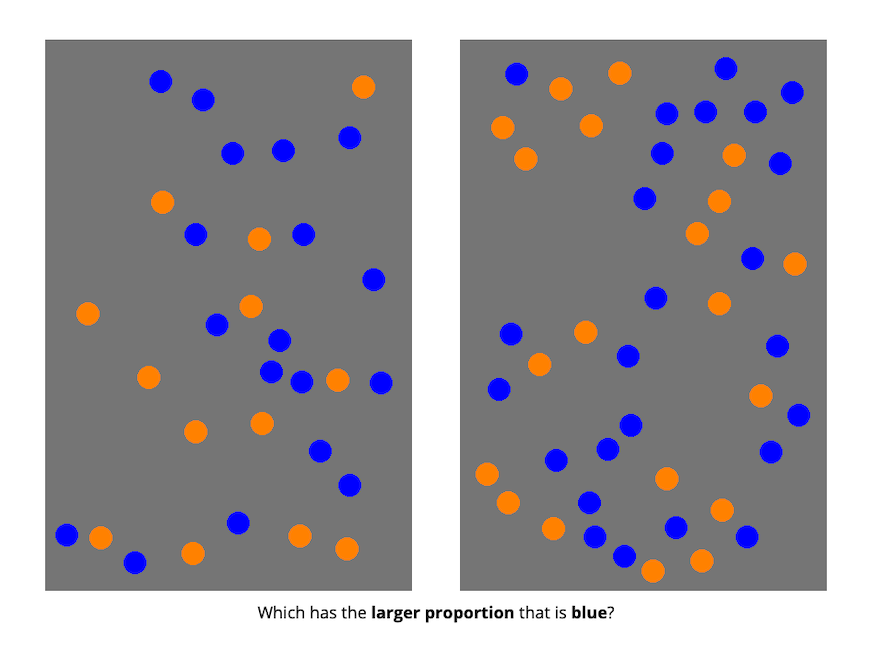
\includegraphics[width=0.5\linewidth]{images_WA10/Probtask_Trial.png}
  \caption{Illustration of Probtask trials.}
  \label{fig:probtask-trial}
\end{figure}

Condition\\
What is not shown in figure \ref{fig:probtask-trial}, is that there were four different conditions that changed what kinds of images the participants saw:\\
-divided blobs: blue and orange were entirely separate\\
-integrated blob: one blob, divided to be part blue and part orange\\
-separated dots: blue and orange dots were on opposite sides of the image\\
-integrated dots: blue and orange dots were intermixed\\

\begin{figure}[H]
  \centering
  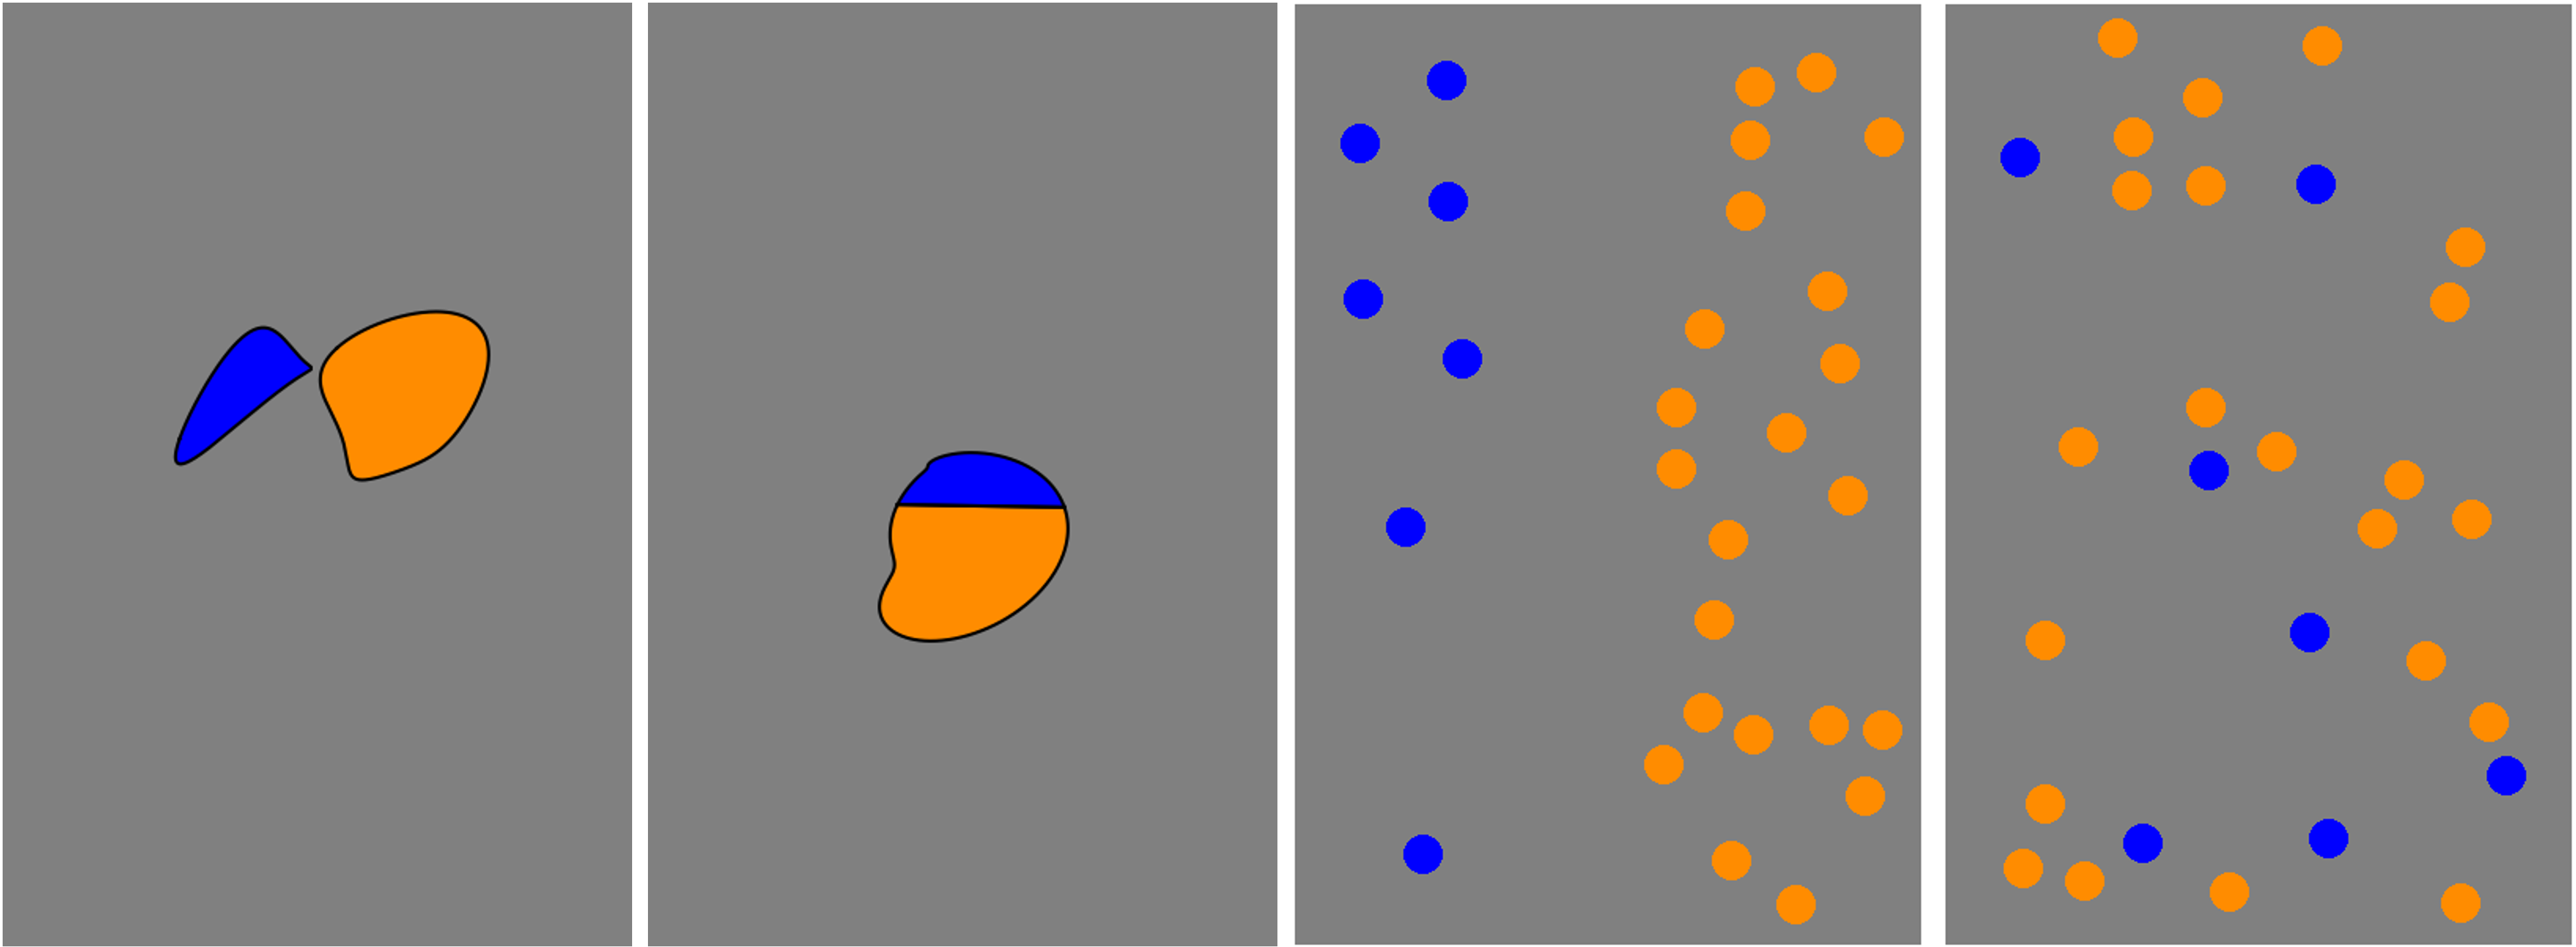
\includegraphics[width=0.5\linewidth]{images_WA10/Probtask_formats.png}
  \caption{Illustration of Probtask formats.}
  \label{fig:probtask-format}
\end{figure}

Note: The conditions in figure \ref{fig:probtask-format} are named as follows(from left to right):Divided Blob, Integrated Blob,Separated Dots, and Integrated Dots
\clearpage

\subsubsection{Data analysis}\label{data-analysis}

We used R {[}Version 4.4.1; @{]} and the R-packages \emph{ggdist} (Version 3.3.2; Kay, 2024), \emph{ggplot2} (Version 3.5.1; Wickham, 2016), \emph{papaja} (Version 0.1.3; Aust \& Barth, 2024) and \emph{tidyverse} (Version 2.0.0; Wickham et al., 2019) for all our analyses.

\section{Results}\label{results}

\begin{enumerate}
\def\labelenumi{\arabic{enumi}.}
\tightlist
\item
  Does average performance vary across format type, ignoring all other aspects of the stimuli?
\end{enumerate}

\begin{figure}
\centering
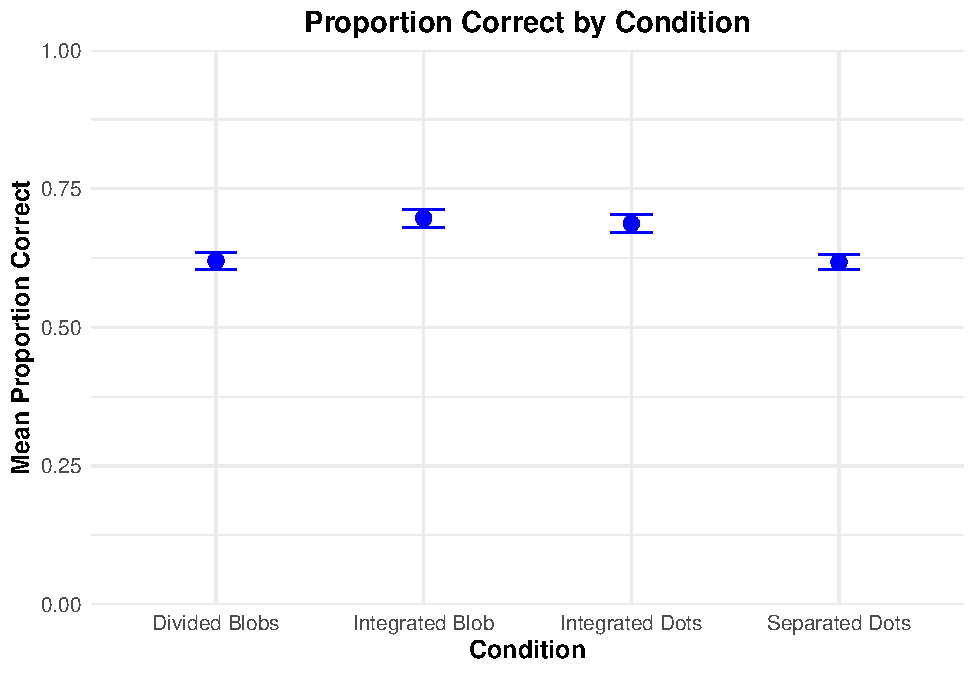
\includegraphics{Sebastian_WA11_files/figure-latex/plot1-1.pdf}
\caption{\label{fig:plot1}Average performance by format type}
\end{figure}

\clearpage

\begin{enumerate}
\def\labelenumi{\arabic{enumi}.}
\setcounter{enumi}{1}
\tightlist
\item
  How are reaction time and accuracy related?
\end{enumerate}

\begin{figure}
\centering
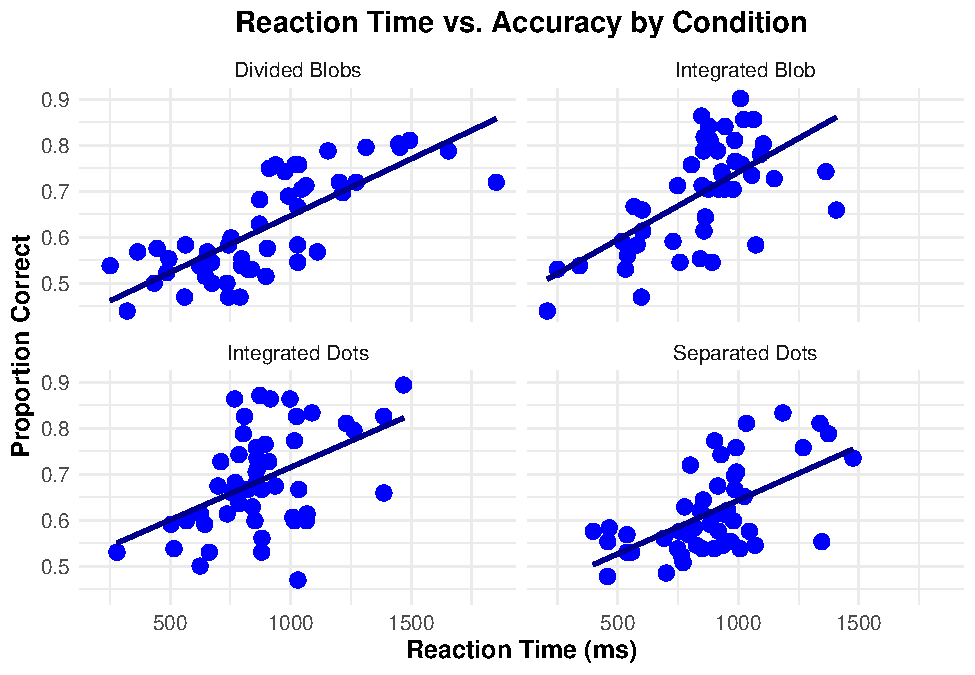
\includegraphics{Sebastian_WA11_files/figure-latex/plot2-1.pdf}
\caption{\label{fig:plot2}Reaction time and accuracy relation}
\end{figure}

\clearpage

\begin{enumerate}
\def\labelenumi{\arabic{enumi}.}
\setcounter{enumi}{2}
\tightlist
\item
  How does numerator congruency interact with format type?
\end{enumerate}

\begin{figure}
\centering
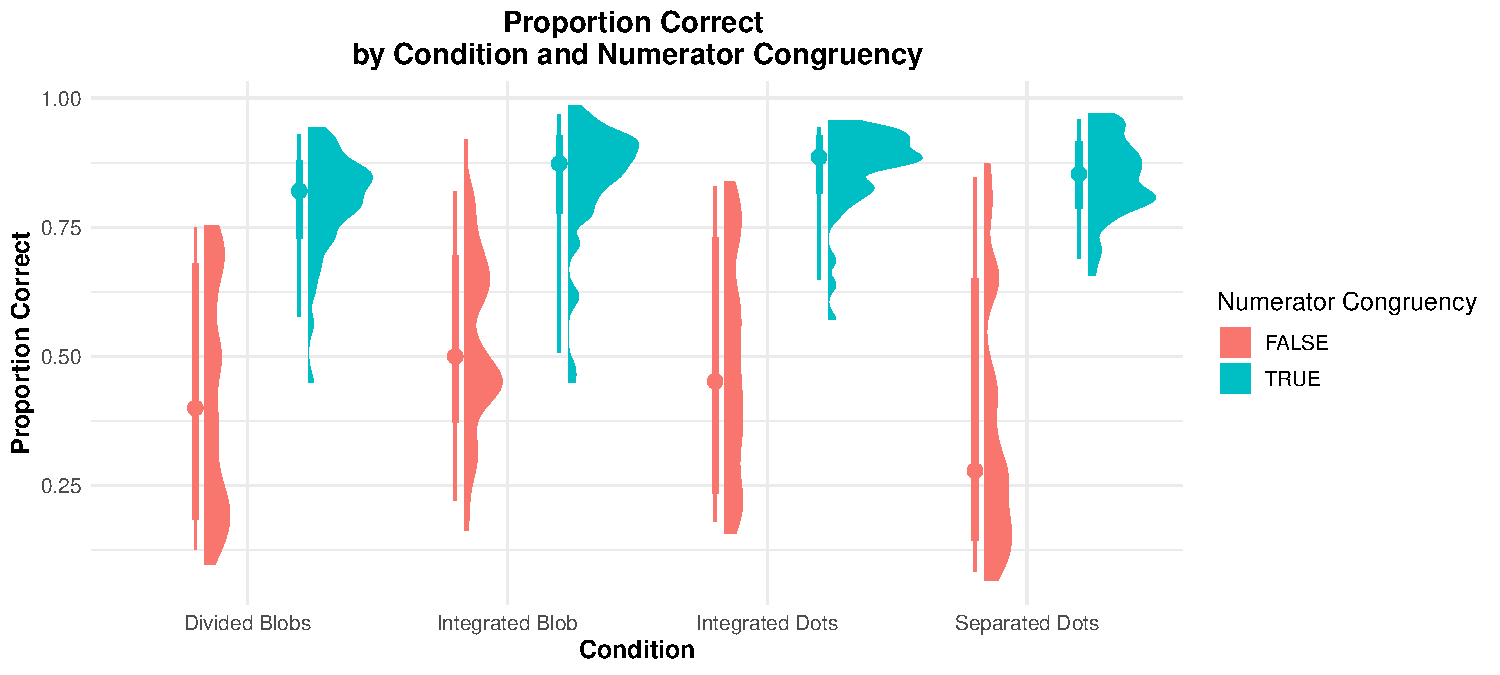
\includegraphics{Sebastian_WA11_files/figure-latex/plot3-1.pdf}
\caption{\label{fig:plot3}How numerator congruency interacts with format type}
\end{figure}

\clearpage

\section{Discussion}\label{discussion}

As per figure \ref{fig:plot1}, participants' average performance was at its best with the integrated blob and dots and was at its worst with the separated/divided blobs and dots.

As shown in figure \ref{fig:plot2}, for all conditions, as reaction time increases, accuracy increases as well

As per figure \ref{fig:plot3}, when there is a numerator congruency, the proportion correct across all format types is higher than when there is not.

\begin{enumerate}
\def\labelenumi{\arabic{enumi}.}
\item
  The most annoying part of this assignment was integrating the old plots into this poster and having to make the adjustments in order to make them ``publication'' ready
\item
  The most satisfying part of this assignment is when you make aesthetic changes on the file and then rendering it to see how much better it makes the poster.
\end{enumerate}

\newpage

\section{References}\label{references}

\phantomsection\label{refs}
\begin{CSLReferences}{1}{0}
\bibitem[\citeproctext]{ref-R-papaja}
Aust, F., \& Barth, M. (2024). \emph{{papaja}: {Prepare} reproducible {APA} journal articles with {R Markdown}}. \url{https://doi.org/10.32614/CRAN.package.papaja}

\bibitem[\citeproctext]{ref-R-ggdist}
Kay, M. (2024). {ggdist}: Visualizations of distributions and uncertainty in the grammar of graphics. \emph{IEEE Transactions on Visualization and Computer Graphics}, \emph{30}(1), 414--424. \url{https://doi.org/10.1109/TVCG.2023.3327195}

\bibitem[\citeproctext]{ref-R-ggplot2}
Wickham, H. (2016). \emph{ggplot2: Elegant graphics for data analysis}. Springer-Verlag New York. Retrieved from \url{https://ggplot2.tidyverse.org}

\bibitem[\citeproctext]{ref-R-tidyverse}
Wickham, H., Averick, M., Bryan, J., Chang, W., McGowan, L. D., François, R., \ldots{} Yutani, H. (2019). Welcome to the {tidyverse}. \emph{Journal of Open Source Software}, \emph{4}(43), 1686. \url{https://doi.org/10.21105/joss.01686}

\end{CSLReferences}


\end{document}
